\documentclass[a4paper,fontsize=12pt]{scrartcl}
\usepackage{Alegreya}
\usepackage{AlegreyaSans}

\usepackage[svgnames,hyperref]{xcolor}
\usepackage{url}
\usepackage{graphicx}

\usepackage{amsmath,amssymb,amsthm}
\usepackage{tikz}
\usetikzlibrary{shapes,arrows}
\usepackage[utf8]{inputenc}

% \usepackage{fullpage}

\usepackage[%
backend=biber,
style=authoryear, % numeric-comp
maxbibnames=10,
url=false,
doi=false]{biblatex}

% make bibliography a bit smaller if necessary
\renewcommand*{\bibfont}{\small}

% \AtEveryBibitem{\clearfield{month}}
% \AtEveryCitekey{\clearfield{month}}

\addbibresource{references.bib}

\usepackage[english=british,threshold=15,thresholdtype=words]{csquotes}
\SetCiteCommand{\parencite}

\newenvironment*{smallquote}
{\quote\small}
{\endquote}
\SetBlockEnvironment{smallquote}

\usepackage[%
unicode=true,
hyperindex=true,
bookmarks=true,
colorlinks=true, % change to false for final
pdfborder=0,
allcolors=DarkBlue,
% plainpages=false,
pdfpagelabels,
hyperfootnotes=true]{hyperref}

\usepackage{todonotes}

\author{}

\date{\today}

\begin{document}

\renewcommand{\thesection}{\Alph{section}}

\setcounter{section}{3} % C1.
\subsection{Project Description}
\label{sec:project-description}
% (Please upload a Project Description as detailed in the Instructions
% to Applicants in no more than 10 A4 pages and in the required
% format. Please refer to the Instructions to Applicants for detailed
% instructions on the required content and format of the Project
% Description.)

\subsubsection*{PROJECT TITLE}

\textbf{Live and interactive parameter-space exploration of environmental simulations with uncertainty quantification} %can differ from grant title and be longer 



\subsubsection*{AIMS AND BACKGROUND}



When systems are disrupted during environmental disasters (for example,
flood, fire, wind, earthquakes) information from
computational simulation can be needed urgently and in an
acceptable format to aid  decision-making by emergency services. 
Meeting such a modelling and simulation 
challenge is not simply a matter of compute power but involves
ideas from software engineering, computational mathematics,
human computer interaction, high performance computing, and data visualisation. Furthermore, all
of these disciplines need to be tightly coupled and benchmarked to
realistic  team-coordination and decision-making scenarios where decision-makers collaborate with modelling experts. 
In particular, 
a crucial aspect of advice provided from modellers to decision makers is to properly quantify and communicate 
the {\em uncertainty} in predictions obtained
by computer simulations. This advice will need to be provided in a time-bound manner and in a context where the computer support may vary dramatically over time due to system outages.

We address this grand
challenge through a {\em live-programming} approach to the software-system development
and deployment of  environmental simulations including uncertainty. 
We will develop new environmental simulations of flood surge and tsunamis which combine sparse grids and uncertainty quantifiction to dramatically increase the speed of delivery of useful predictions and the uncertainty associated with those predictions.
We will deploy  ``live"  distributed
computing infrastructure to {\em rapidly prototype} the human interface to these new environmental simulations and to effectively transform the
traditional, batch-oriented modality of environmental simulation into a highly-interactive one. We will 
evaluate team coordination and decision-making under uncertainty by field trials of our prototype systems in the setting of a mock-reality game and by analysing the protocols of live-coding optimisation of the software system during those field trials. From these protocols, identifiable states and transitions between those states will be used to iterate our software-system development. 

Our vision is that decision makers
will be able to examine many different environmental disaster scenarios in a short space of
time, even with computationally-expensive models. This will enable
them to develop an intuitive understanding of the uncertainty
relationships in the system---from uncertainties in input data through
to representations of uncertainty in model outputs. The importance of
such a human-in-the-loop workflow has been expressed
by~\textcite{pike_science_2009} in the following quote: ``it is through the interactive
manipulation of a visual interface---the analytic discourse---that
knowledge is constructed, tested, refined and shared.''

Although the mathematical and computational tools we will employ in
this project are generalisable to any modelling workflow, we will
focus on specific application domains where (a) the model is (computationally)
complex, (b) uncertainty is significant and (c) decisions are
time-sensitive. Specifically, we will build interactive interfaces for
 storm-surge and tsunami flood modelling. 

The mathematical component of this project will be based on new
mathematical developments combining sparse grids and uncertainty
quantification. One of the main difficulties in current models is the
high dimensional spaces involved, both in the parameter and
domain spaces. Sparse grids~\parencite{BungartzGriebel2004} are
well-known to reduce the effects of the so called ``curse of
dimensionality", whereby the cost of computation increases
exponentially with the dimension of the model.
We have recently found new ways to incorporate gradient
information and multi-fidelity models into sparse grid
approximations~\parencite{deBaarHarding2015,Jakeman2015,deBaarRDM2015} and we will be
deploying this knowledge in our construction of a suite of surge-tsunami models to simulate
environmental disasters with uncertainty quantification.


Computational decision support systems for disaster management
have existed for many decades~\parencite{wallace_decision_1985}, and
advances have been made both in incorporating
uncertainty~\parencite{thompson_social_2014-1,neale_navigating_2015}
and providing real-time output~\parencite{yu_support_2006}. More recently, 
mixed-reality game scenarios have been used to understand and optimise human-agent 
collaboration for disaster response~\parencite{ramchurn2016human}.
In our project plan we will follow a similar approach and will employ mock-game scenarios to examine and understand the nature of decision making with expert modelling support. In a novel twist, we will run these games together with live-coding optimisation and tuning of the software system and the underlying computational platform. By analysing the protocols of these live optimisations, we will accumulate data to feed into redesign of the software interface and to understand the time requirements and controls needed for the computational platform.


This project will provide the following discoveries and benefits:
\begin{enumerate}

\item a suite of interactive, real-time modelling tools for surge-tsunami flood disasters which combine
full simulations with coarse-grid, rough simulations to quantify
uncertainty, optimised for human exploration


\item a ``live software engineering" approach to the development, deployment 
and optimisation of these interactive software systems; 

\item models of group interaction scenarios for decision-making 
 with expert modelling support; from these models, empirical estimates of  the 
time constraints that such scenarios place impose on software and computer system requirements and the live controls needed to run them effectively in volatile contexts

\item interactive information visualisations of simulation predictions
together with uncertainties
 

\end{enumerate}

In the wider picture, this research is significant because it aims to unlock the power of
sophisticated
computational simulation for interactive use. Although we concentrate
our research on simulation support for disaster response, the
ultimate potential of this work is to eventually empower domain
experts from a broad range of areas to better use the high-performance
computing power which is now available to them. We envision a future
where performing a complex flood model or disaster simulation is as
interactive and \emph{alive} as flicking through photos on an iPad.




\subsubsection*{RESEARCH PROJECT}
% - Describe how the research is significant and how it addresses an important problem
% - Describe how the Proposal meets the objectives of the Discovery Projects scheme
% - Describe how the anticipated outcomes will advance the knowledge base of the discipline and
%   how the Proposal aims and concepts are novel and innovative
% - Outline the conceptual framework, design and methods and demonstrate that these are
%   adequately developed, well integrated and appropriate to the aims of the Proposal. Include
%   research plans and proposed timelines
% - Detail what new methodologies or technologies will be developed in the course of the research
%   and how they will advance knowledge
% - Outline the feasibility of the project, in terms of design, budget and proposed timeline
% - If the rationale for some of the Proposal rests upon manuscripts that are still in the process of
%   being published, or on results of work that may not be available to assessors, include a
%   summary of the relevant work
% - Describe the expected outcomes and likely impact of the proposed research
% - Describe how the Proposal might result in national or international economic, commercial,
%   environmental, social and/or cultural benefits
% - If the research has been nominated as focussing upon a topic or outcome that falls within one
%   of the Science and Research Priorities, describe the potential for the project to contribute to the associated Priority Goals.

The January 2011 Brisbane River floods in south-east Queensland cost
32 lives and caused 2.5~billion dollars worth of
damage~\parencite{vandenhonert_2011_2011}. In the days leading up to
these events, a key issue facing authorities was incorporating their
\textbf{uncertainty} about the preceding fortnight's rainfall into the
modelling. In their report on the causes, impacts and implications of
the floods, \textcite[p1170]{vandenhonert_2011_2011} concluded:
\blockquote{whilst the dam operators were acting in accordance with
  the operations manual for the dam, their modelling did not take
  account of forecast rainfall in determining the predicted dam water
  level, and this resulted in a sub-optimal water release strategy.
  Employing tools for decision making under uncertainty would have
  resulted in a different water release strategy.} 
At the other end of
the environmental spectrum, bushfire model predictions are similarly
\textquote[\cite{alexander_limitations_2013} p375]{fraught with
  uncertainty}. As Australia's climate changes and extreme weather
events become more common, there is a significant need for better ways to
gather timely insights from modelling in the presence of uncertainty and to communicate those insights to 
decision makers and emergency services.

Computational modelling and simulation is an invaluable support tool for disaster respon\-se,
 allowing  emergency services personnel to explore 
what might happen in the immediate future 
under various scenarios. But these model simulations can be fraught with uncertainty: 
some of their {\em input parameters}  may be well
known (possibly from reliable sensor data), while others are known only approximately, and others still may
only be guessed at. Even given perfect input data, the models themselves entail assumptions and numerical approximations which bound the reliability of their predictions. 

Slightly more formally, suppose that we have a mathematical model $M_{\mathbf{p}}$
parameterised by the vector $\mathbf{p}\in\mathcal{P}$. For example, $M_{\mathbf{p}}$ may
be a parameterised partial differential equation %(PPDE) 
in a storm
surge model. For each $\mathbf{p}$ we suppose the model is
well-defined and there exists a unique function
\begin{equation}
  \label{eq:1}
  u_{\mathbf{p}}(\mathbf{x})\, \quad \mathbf{x}\in\Omega
\end{equation}
which is a solution to the model problem, that is $M_{\mathbf{p}}(u_{\mathbf{p}})=0$.
Sometimes the goal of the modeller is to better understand the relationship
between $\mathbf{p}$ and some lower-dimensional quantity of interest
$Q(u_{\mathbf{p}})$, such as the relationship between a particular rainfall scenario and the maximum storm surge levels at particular geographical locations. In order to achieve such understanding, repeated executions of the model are often required with an expert analysis of the outputs of each stage and selection of the next parameter set based on an assessment of those outpus. Such repeated model executions can also be used to estimate the {\em uncertainty} in any given set of predictions of 
$Q(u_{\mathbf{p}})$. Through the process
of trying different model parameterisations, the scientist is able to
build up an understanding of the \emph{general} relationship between
$\mathbf{p}$ and $Q(u_{\mathbf{p}})$, including the areas of the
parameter space $\mathcal{P}$ which have the greatest influence on the
result and which
types of uncertainty have the greatest impact on the certainty of the
results.

%or to find the parameter choice $\mathbf{p}$
%which optimises $Q$. %over all $\mathbf{x}$.
%This high-level description of the ``model selection/optimisation''
% workflow 
%(shown
%graphically in Figure~\ref{fig:general-fb-loop})
 %lies at the heart of
%a great deal of modern science.
%\begin{figure}
 % \centering
  %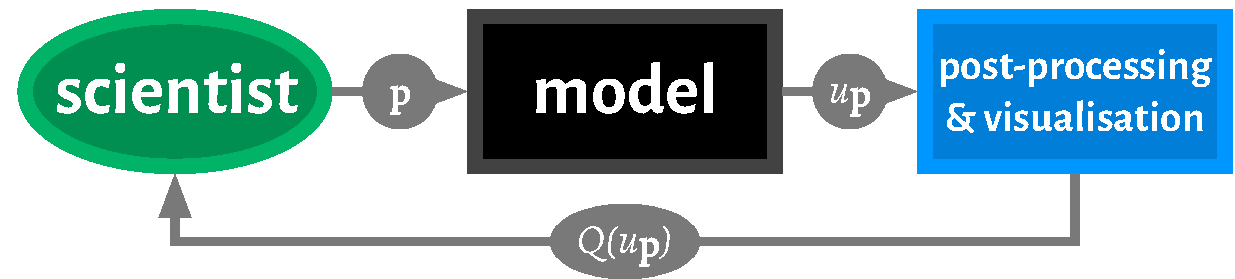
\includegraphics[width=.6\textwidth]{figures/general-fb-loop.pdf}
  %\caption{The human-in-the-loop modelling workflow. A scientist
    %selects an initial parameter $\mathbf{p_0}$ for their model,
    %examines the model output $Q(u_{\mathbf{p}})$, and either accepts
    %the output of the model or re-runs the model with a different
    %choice of the parameter $\mathbf{p_1}$.}
  %\label{fig:general-fb-loop}
%\end{figure}
%There are many ways of finding an optimal $\mathbf{p}$, from 
%trial-and-error experimentation to expert judgement through to fully-automated algorithmic
%optimization procedures. Often there are ways to optimise $\mathbf{p}$
%algorithmically, although these methods often introduce new parameters (the
%arguments of the function being optimised) which must be selected by the
%scientist. 
%As a result, this feedback loop will often require many
%iterations, with a scientist-in-the-loop, evaluating the results
%of the model (possibly through visualising the model output) and
%choosing a parameter update $\Delta\mathbf{p}$ at each step.
% (see
%Figure~\ref{fig:unrolled-fb-loop}). 
%Each step through this loop
%provides feedback to the scientist about the response of the system to
%a particular value of $\mathbf{p}$ --  for example, the maximum storm
%surge level under a particular rainfall scenario. 

%\begin{figure}
% \centering
%  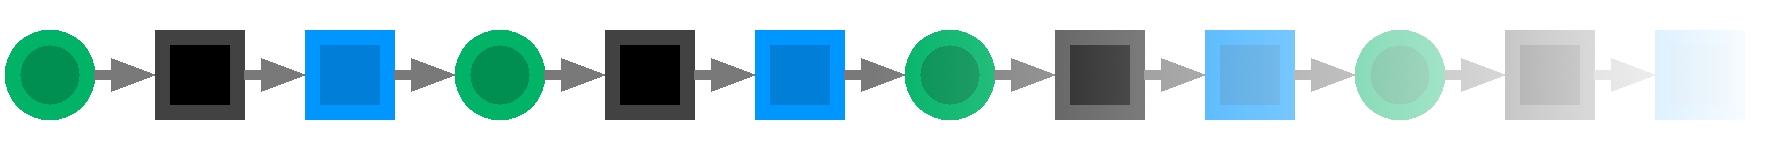
\includegraphics[width=\textwidth]{figures/unrolled-fb-loop.pdf}
%  \caption{If the modelling \& post-processing/visualisation steps can
%    be performed sufficiently quickly, then the scientist can explore
%    the $\mathbf{p} \rightarrow Q(u_{\mathbf{p}})$ relationship
%    \emph{interactively}, with the all the associated benefits for
%    exploratory analysis.}
%  \label{fig:unrolled-fb-loop}
%\end{figure}

From a workflow perspective, the productivity of the modeller/scientist can be 
proportional to the rate at which they can explore the
$\mathbf{p} \rightarrow Q(u_{\mathbf{p}})$ relationship. Any latency
improvements in this feedback loop will translate into productivity
gains~\parencite{liu_effects_2014}.
If the model parameters $\mathbf{p}$ and inputs $\mathbf{x}$ are known
precisely and the quantity $Q(u_{\mathbf{p}})$ is cheap to calculate
and easy to interpret, then the task is simple: provide the scientist
with an interface for manipulating $\mathbf{p}$ and set them loose.
However, for real-world models (such as those used in flood/storm
surge/bushfire modelling) this is often not the case. There are \textbf{three
primary challenges}:
\begin{enumerate}
\item \emph{The model may not provide a way to express uncertainty in
    the inputs}. Many models do not provide methods for including
  uncertainty information in their inputs, as was the case in the
  Lockyer valley example.
\item \emph{The quantity $Q(u_{\mathbf{p}})$ may not be cheap to
    calculate}. Many
  sophisticated models require non-trivial computing resources to evaluate. These compute resources may be
  difficult to secure, with submitted jobs having to wait in a queue, and may
  take a long time to compute even when the resources are available.
  This is especially problematic in a disaster-response scenario,
  where an approximately correct answer provided in a short time is
  significantly more useful than a perfect answer provided after it is
  too late to act on.
\item \emph{The quantity $Q(u_{\mathbf{p}})$ together with estimates of its uncertainty may not be easy to
    interpret}. Oftentimes this is a visualisation problem---
  the mapping $\mathbf{p} \rightarrow Q(u_{\mathbf{p}})$ may be high-dimension\-al,
  and presenting that to a decision-maker, particularly when combining it with its uncertainty estimates, may not be straightforward.
\end{enumerate}
%\begin{figure}
 % \centering
  %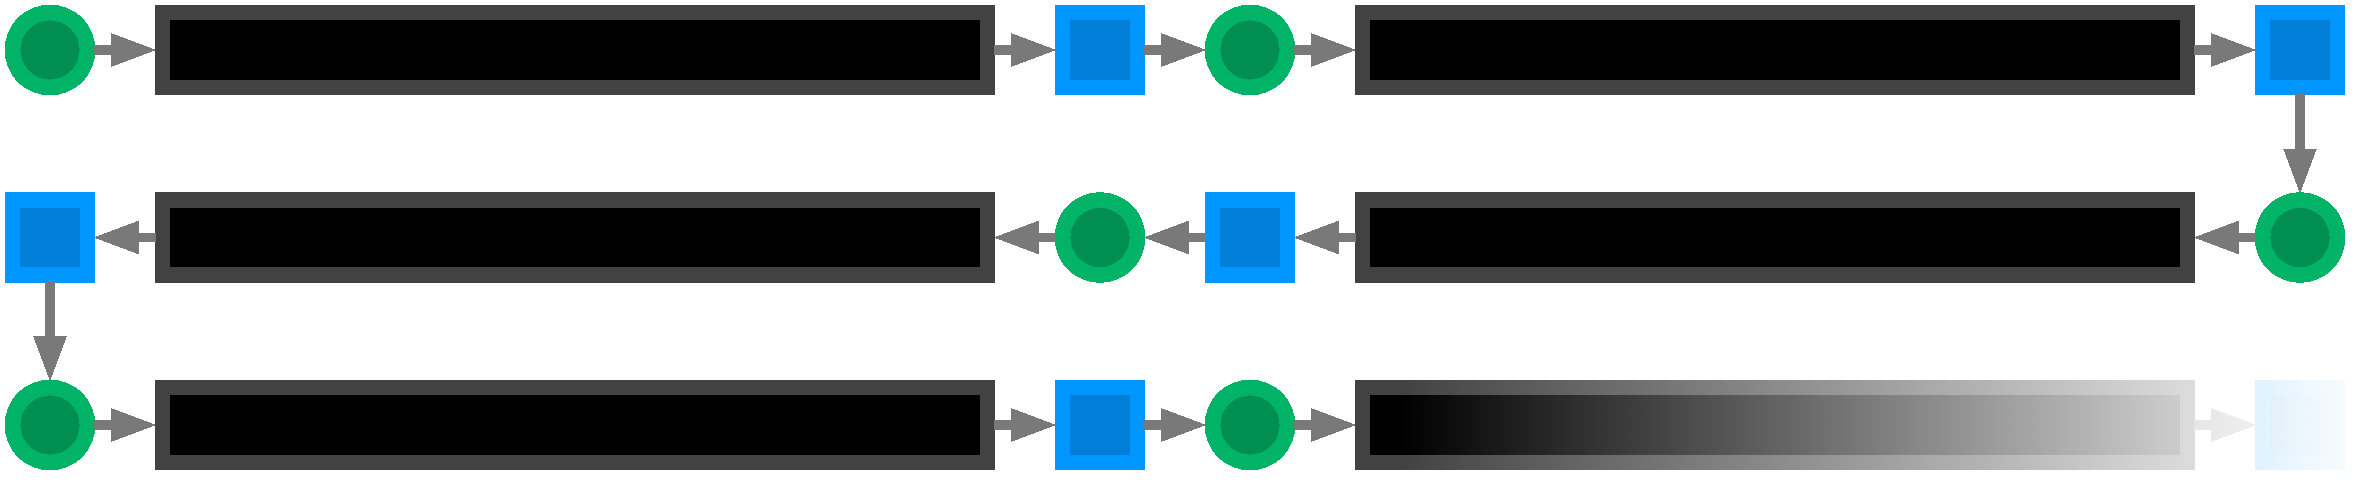
\includegraphics[width=\textwidth]{figures/long-fb-loop.pdf}
  %\caption{If the model is computationally expensive to run, then the
   % workflow is dominated by waiting for the model to finish. This
    %results in lower productivity---not only due to the time spent
    %waiting for the model, but also because of the temporal separation
  %between the selection of a new parameter $\mathbf{p}$, and seeing
 % its impact on the results of the model.}
 % \label{fig:long-fb-loop.pdf}
%\end{figure}

In this project, by accelerating the feedback loop between $\mathbf{p}$ and
$Q(u_{\mathbf{p}})$, together with estimates of its uncertainty, we will give
the scientist the ability to interactively \emph{explore} the
connection (and the associated uncertainty) between the different
dimensions of $\mathbf{p}$ and the overall response of the system.
By understanding the human-factors and systems-level time constraints on the delivery of useful information in
disaster-response settings, we will be able to specify timing requirements on our model simulations.
By developing software that is time-constrained and time-aware, we will be able to provide decision makers
with information when it is needed and with an estimate on the uncertainty of that information. 

%Ultimately, the scientist needs an \textbf{interactive interface} for
%gleaning insights from their models in the presence of these
%challenges.

Our vision for dealing with the above challenges
involves using sparse grids and reduced basis models 
combined with live modification
of simulation parameters, dynamic steering of computational resources and
interactive visualisation. Specifically:
\begin{enumerate}
\item \emph{(Uncertainty in inputs):} By using sparse grids and reduced basis models to precompute
  a surrogate model, existing models (which may not
  provide a way to encode uncertainty information) can be used as
  ``black boxes'', and expectation integrals over subsets of the
  parameter space $\mathcal{P}$ (which are important for quantifying
  uncertainty) can be efficiently estimated from the
  surrogate model $\tilde{u}_{\mathbf{p}}(\mathbf{x})$. This has
  significant benefits over classical Monte Carlo methods when the
  integrand is sufficiently
  smooth~\parencite{JakemanRoberts2013,FranzelinDiehlPfluger2014}.

\item \emph{(Cheap to calculate):} For many problems the computation of solutions 
  $u_{\mathbf{p}}(\mathbf{x})$ to the model $M_{\mathbf{p}}$ can be done 
  cheaply using the combination technique over the domain
  $\mathbf{x}\in\Omega$}.
  One may also develop reduced basis models to achieve the same outcome. For our disaster response scenarios, the concept of ``cheapness" will be reframed as one of ``timeliness": we will build systems which guarantee modelling results within particular timeframes of relevance to human factor processes in group decision making.

\item \emph{(Easy to interpret):} Since a sparse grid sampling of $\mathbf{p}\in\mathcal{P}$ enables a fast 
  and efficient exploration of parameter space, there is more time for
  visualisation and post-processing in an interactive interface, which
  allowing richer ensembles of visualisation techniques to assist the
  decision-maker in interpreting the results of the model.
\end{enumerate}

%\begin{figure}
 % \centering
  %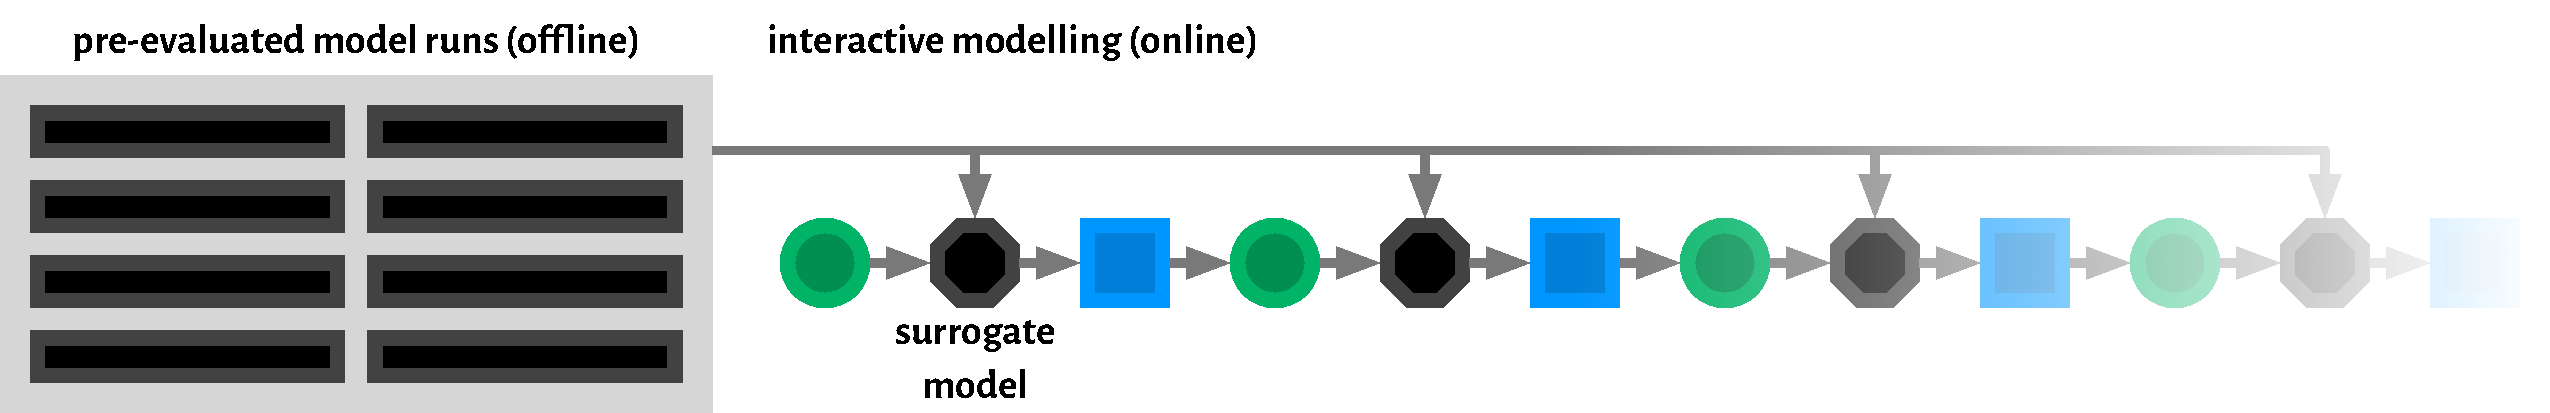
\includegraphics[width=\textwidth]{figures/sg-surrogate-model-fb-loop.pdf}
  %\caption{Using the sparse grids and reduced basis models, the computationally
   % expensive model calculations can be done ahead-of-time and used to
    %construct a surrogate model which can be used to re-claim the
    %interactive workflow of Figure~\ref{fig:unrolled-fb-loop}}.
  %\label{fig:sg-surrogate-model-fb-loop}
%\end{figure}

%Impact: new algorithms, software, high performance computer systems
%and visualisation techniques for time-bound environmental simulation
%with uncertainty. New software tools for the simulation of flood
%surges and tsunami. New methodologies for rapid and agile software
%development and usability using live programming. New knowledge of
%human-in-the-loop requirements for support systems in the context of
%environmental disaster management. New algorithms, software, high
%performance computer systems and visualisation techniques for
%time-bound environmental simulation with uncertainty. New software
%tools for the simulation of flood surges and tsunami. New
%methodologies for rapid and agile software development and usability
%using live programming. New knowledge of human-in-the-loop
%requirements for support systems in the context of environmental
%disaster management.





\noindent{\bf Sparse-Grids and Uncertainty Quantification}\\

The mathematical component of this project will be based on new
mathematical developments combining sparse grids~\parencite{BungartzGriebel2004}, 
reduced basis methods~\parencite{LiebermanEtal2010,Peherstorfer2013,ChenSchwab2015}
and uncertainty quantification. 
One of the main difficulties in the study of current scientific models is
the high dimensional spaces involved, often both in the parameter and
domain spaces, $\mathcal{P}$ and $\Omega$ respecitvely. 
This is a significant barrier for the timely evaluation of models due to the 
``curse of dimensionality'' in which the cost scales exponentially with dimension.
By using sparse grids and reduced basis models we will be able to compute
{\em surrogates of the full problem} which have lower dimensionality and are thus cheaper  
to compute whilst maintaining a high order of accuracy.
For example, a general approach would be to find a lower dimensional manifold 
of the parameter space $\mathcal{Q}\subset\mathcal{P}$ over which the 
model is most sensitive using reduced basis methods.
A sparse grid surrogate of the model over $\mathcal{Q}$ can then be 
computed in an offline phase, so that in an online phase model solutions
can be efficiently estimated using the surrogate model.
For many problems sparse grids can also be used over $\Omega$ when  
computing solutions to the full model. 
This will significantly speed up the computation of a reduced basis.
We will compute sparse grid solutions via the
``combination technique''~\parencite{Griebel1990}. 
Figure~\ref{fig:sparse_grids} depicts the combination technique, the
equivalent sparse grid and the corresponding full grid. 

\begin{figure}
  \centering
  % Brendan: combination grid, sparse grid, fullgrid figure

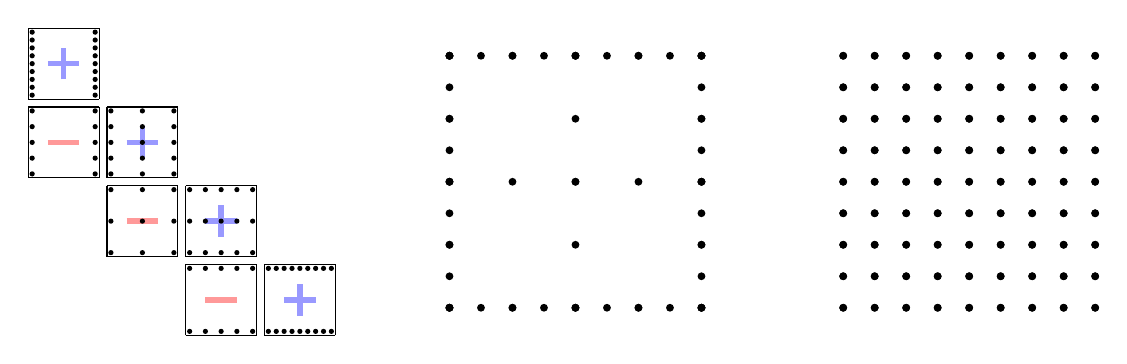
\begin{tikzpicture}%[scale=0.8]
%\scriptsize
%%% Draw squares around component grids
\foreach \i in {1,...,4}
{
	\pgfmathtruncatemacro{\x}{(\i - 1)};
	\draw[] (0.05+1.0*\x, 3.05-1.0*\x) -- (0.05+1.0*\x+0.9, 3.05-1.0*\x) {};
	\draw[] (0.05+1.0*\x, 3.05-1.0*\x) -- (0.05+1.0*\x, 3.05-1.0*\x+0.9) {};
	\draw[] (0.05+1.0*\x+0.9, 3.05-1.0*\x) -- (0.05+1.0*\x+0.9, 3.05-1.0*\x+0.9) {};
	\draw[] (0.05+1.0*\x, 3.05-1.0*\x+0.9) -- (0.05+1.0*\x+0.9, 3.05-1.0*\x+0.9) {};
	%%% optional plotting of coefficients
	\draw[blue!40,line width=0.7mm] (0.5+1.0*\x-0.2, 3.0+0.5-1.0*\x) -- (0.5+1.0*\x+0.2, 3.0+0.5-1.0*\x);
	\draw[blue!40,line width=0.7mm] (0.5+1.0*\x, 3.0+0.5-1.0*\x-0.2) -- (0.5+1.0*\x, 3.0+0.5-1.0*\x+0.2);
}
\foreach \i in {1,...,3}
{
	\pgfmathtruncatemacro{\x}{(\i - 1)};
	\draw[] (0.05+1.0*\x, 2.05-1.0*\x) -- (0.05+1.0*\x+0.9, 2.05-1.0*\x) {};
	\draw[] (0.05+1.0*\x, 2.05-1.0*\x) -- (0.05+1.0*\x, 2.05-1.0*\x+0.9) {};
	\draw[] (0.05+1.0*\x+0.9, 2.05-1.0*\x) -- (0.05+1.0*\x+0.9, 2.05-1.0*\x+0.9) {};
	\draw[] (0.05+1.0*\x, 2.05-1.0*\x+0.9) -- (0.05+1.0*\x+0.9, 2.05-1.0*\x+0.9) {};
	%%% optional plotting of coefficients
	\draw[red!40,line width=0.7mm] (0.5+1.0*\x-0.2, 2.0+0.5-1.0*\x) -- (0.5+1.0*\x+0.2, 2.0+0.5-1.0*\x);
}
%%% Combination grids
\foreach \i in {1,...,18} %2*9
{
	\pgfmathtruncatemacro{\y}{(\i - 1) / 2};
	\pgfmathtruncatemacro{\x}{\i - 1 - 2 * \y};
	\node[fill,circle,scale=0.2] at (0.1+0.8*\x,3.1+0.1*\y) {};
	\node[fill,circle,scale=0.2] at (3.1+0.1*\y,0.1+0.8*\x) {};
}
\foreach \i in {1,...,15} %3*5
{
	\pgfmathtruncatemacro{\y}{(\i-1)/3};
	\pgfmathtruncatemacro{\x}{\i-1-3*\y};
	\node[fill,circle,scale=0.2] at (1.1+0.4*\x,2.1+0.2*\y) {};
	\node[fill,circle,scale=0.2] at (2.1+0.2*\y,1.1+0.4*\x) {};
}
\foreach \i in {1,...,10} %2*5
{
	\pgfmathtruncatemacro{\y}{(\i-1)/2};
	\pgfmathtruncatemacro{\x}{\i-1-2*\y};
	\node[fill,circle,scale=0.2] at (0.1+0.8*\x,2.1+0.2*\y) {};
	\node[fill,circle,scale=0.2] at (2.1+0.2*\y,0.1+0.8*\x) {};
}
\foreach \i in {1,...,9} %3*3
{
	\pgfmathtruncatemacro{\y}{(\i - 1) / 3};
	\pgfmathtruncatemacro{\x}{\i - 1 - 3 * \y};
	\node[fill,circle,scale=0.2] at (1.1+0.4*\x,1.1+0.4*\y) {};
}
%%% Sparse grid
\foreach \i in {1,...,18} %2*9
{
	\pgfmathtruncatemacro{\y}{(\i - 1) / 2};
	\pgfmathtruncatemacro{\x}{\i - 1 - 2 * \y};
	\node[fill,circle,scale=0.3] at (5.4+3.2*\x,0.4+0.4*\y) {};
	\node[fill,circle,scale=0.3] at (5.4+0.4*\y,0.4+3.2*\x) {};
}
\foreach \i in {1,...,15} %3*5
{
	\pgfmathtruncatemacro{\y}{(\i-1)/3};
	\pgfmathtruncatemacro{\x}{\i-1-3*\y};
	\node[fill,circle,scale=0.3] at (5.4+1.6*\x,0.4+0.8*\y) {};
	\node[fill,circle,scale=0.3] at (5.4+0.8*\y,0.4+1.6*\x) {};
}
%%% Full grid
\foreach \i in {1,...,81} %9*9
{
	\pgfmathtruncatemacro{\y}{(\i - 1) / 9};
	\pgfmathtruncatemacro{\x}{\i - 1 - 9 * \y};
	\node[fill,circle,scale=0.3] at (10.4+0.4*\x,0.4+0.4*\y) {};
	\node[fill,circle,scale=0.3] at (10.4+0.4*\y,0.4+0.4*\x) {};
}
\end{tikzpicture}  
  \caption{Combination grids on the left (with coefficients, marked with
    a blue plus for $+1$ and red minus for $-1$), sparse grid in the
    middle, full grid on the right.}
  \label{fig:sparse_grids}
\end{figure}

Propagating uncertainty in scientific models which are high dimensional 
and/or expensive to compute is a significant challenge.
For models which are not stochastic in nature, and thus have no means
of directly quantifying uncertainty, one must typically estimate statistical 
moments via quadrature rules. Fo high dimensional problems 
it has been shown that sparse grids can estimate these moments faster 
and more accurately than traditional Monte Carlo methods when the 
probability density functions are sufficiently smooth~\parencite{JakemanRoberts2013,FranzelinDiehlPfluger2014}.
Despite the advantages of reduced basis methods, the manifold $\mathcal{Q}$
is still sufficiently high dimensional that the quantification of uncertainty
is a challenge. As such we will continue to develop numerical methods for 
uncertainty quantification through the study of highdimensional approximations.
Replacing the full model with a reduced basis model also adds additional 
uncertainties. One needs to have some idea what the model outcomes may be 
for parameters not lying on the lower dimensional manifold $\mathcal{Q}$.
By using ensemble methods and gradient enhanced 
approximation~\parencite{deBaarHarding2015,Jakeman2015} we will
propogate these uncertainties through the reduced basis model 
to provide a complete picture of uncertainties in the full model problem.
Incorporating ideas from ``Kriging" (Gaussian process regression), a feature of which is having 
confidence intervals over an interpolant, together with sparse-grid interpolation,
we will be able to express uncertainties explicitly in the surrogate model.\\


\noindent{\bf Live-Coding of Scientific Simulation}\\


Live coding is a term which has been used to denote
systems which support the direct intervention of the programmer in a
program's run-time state. It can be thought of as an extreme version of
just-in-time (JIT) programming where there is a direct correlation
between a program's representation and its execution. An example of
this is the visual language Self~\parencite{ungar_self_1987} where
each visual element in the language is a directly programmable object.
As the ambition of live-coding has grown, support systems and languages
 have evolved to have access to clock-time and other
computer-system properties at a language level in order to, for
example, create, modify and interact with music and cyberphysical devices
in real time. 
Such an approach has been 
termed ``Programming with Time"~\parencite{sorensen2010programming}. This project will make use of the {\it Extempore} software environment~\parencite{sorensen_extempore} which has been shown to be able to harness  a traditional batch-mode scientific simulations, written in the C language, and visualise and modify that simulation interactively, and in real-time, with negligible performance overhead (Swift et al., paper title, Journal of Supercomputing Frontiers and Innovations, next issue, to appear in 2016). This software environment will be a key tool for this project as it ill allow us to fine tune our suite of simulation software for disaster response scenarios.\\



\noindent{\bf From Disaster-Response Human-Factors Optimisation to Software Development}\\

% GOMS model for co-operative scenarios where someone wants
% information, and someone is trying to present it to them

% it's about chunking complex tasks c.f. beginning-middle-end

% the goal: quantitative requirements on the time bounds, which has
% implications for the design of the systems

Similar to ~\parencite{ramchurn2016human} we will employ game scenarios to understand and optimise 
collaboration for disaster response~\parencite{ramchurn2016human}.
However, our focus will be on  decision-maker/modeller communication rather than human/agent communication and our game scenarios will take place while software and systems parameters, particularly the human-computer interface, visualistaions and system configuration, are being tuned in real time by a live coder.  In a novel approach, the protocols obtained from this live coding will then be analyse to determine macro, ``chunking" states, of human action and transitions between those states. We have recently used similar approaches to understand the real-time actions of single live-coders in computer music performance~\parencite{swift2014coding} and the macro-gesture states of group computer musicians using iPads~\parencit{martin2015tracking}. In both of these studies, transition matrices derived from interaction protocols were able to yield insights into the artistic process. In the case of the present project, data from the interaction protocols of the live-coder will be feed back into redesign of the software interface and the controls needed for the computational platform.

By way of one simple example, we imagine that, perhaps, the live coder finds that a particular measure of uncertainty, Measure-A, is routinely requested by a decision maker after another particular measure, Measure-B. The live coder could tune up the software in real time so that these two measures could be presented together. The interaction protocols in this instance might reveal insights into the {\em context} where these two measures were requested one after the other and the software might be redesigned to recognise that context and to make the two measures accessible in that context. For another simple example, the live-coding protocol might show that data processing needed to be occasionally shifted from one part of a cloud resource to a local cluster. Examination of these instances could impact on the computer systems settings needed to properly deploy these simulations. (Note that our approach to protocol analysis will go well beyond simple examples like these and will use matrix theory to derive insights into the nature of state transitions across entire protocols and across test participants.)\\


\noindent{\bf High-Performance Computing Systems Support}\\

A reliance on high performance computing for the evaluation of scientific 
models provides additional challenges to the technical side of the project. 
Specifically, our algorithms must be highly scalable and robust to errors and faults in the computer system layer.
There have been many recent developments in both highly-scalable algorithms 
and the sparse grid combination technique which will be of use for this and,
additionally, it has been recently shown that such computations can be made robust~\parencite{HardingHLS2015,AliEtal2015}.
By leveraging and continuing to develop these algorithms we can ensure that
the components of our software system that require high performance 
computing resources will be both scalable and robust.

In this project we will leverage on-demand compute resources, such as
the Amazon AWS cloud~\parencite{amazon_aws} and the National Compute
Infrastructure NCI Cloud~\parencite{nci_cloud}. Using these cloud
services will further improve the project's ability to deliver timely
results in high-pressure and time-critical decisionmaking scenarios.

Once again, we emphasise that our approach to live-coding of test software is a novel aspect of our methodology. The {\em Extempore} tool that we have developed has been shown to be able to harness and steer scientific simulation in real time. In this part of the project, we will apply this tool to the real-time steering of the computer systems layer itself.\\


\noindent{\bf Interactive visualisation of environmental forecasts with uncertainty}\\

Similar to the impact of visualy presented geodata on decision making~\parencite{kinkeldey2015evaluating}, the particular visualisations of 
uncertainty in our environmental models will need to be systematically evaluated with 
human participants. Here we will adopt traditional human-factors trials with non-expert participants together with qualitative feedback from emergency services experts. We will solicit qualitative feedback from expert participants from emergency authorities in our local area including ACT Emergency Service, Geosciences Australia, the Australian Maritime and Safety Authority and the Australian Federal Police. Perspectives offered by this participant pool will be important in extrapolating our study results to real world disaster-management. 



% TODO Need to say something about the exemplar/case studies here.

% try to chunk the interactions and thought processes involved in
% real-time decisionmaking


% interface should be aware of time, just like Extempore. so it's a
% contribution to human-in-the-loop programming

% Why is interactivity important? Because it takes the abstract
% connection between $\mathbf{p}$ and $Q(u_{\mathbf{p}})$ and makes it a malleable,
% responsive, tactile one. What happens when I change $\mathbf{p}$ a little bit
% in this direction? What about in \emph{that} one? How about \emph{both
%   together?}

\subsubsection*{ROLE OF PERSONNEL}
% - Summarise the role, responsibilities and contributions of each Chief Investigator (CI) and Partner Investigator (PI)
% - Summarise the roles and levels of involvement of other Participants, for example, technical staff, Research Associates and other personnel
% - Describe how each Participant will ensure they have the ‘time and capacity’ to undertake the proposed research, taking into account any other grants or roles that they hold.

%The personnel on this grant cover the key research areas discussed in
%the \emph{Research Project} section of this application:
%
%\begin{itemize}
%\item \textbf{Steve Roberts}: uncertainty quantification, sparse grids, flood
%  modelling
%\item \textbf{Markus Hegland}: sparse grids
%\item \textbf{Peter Strazdins}: sparse grids, distributed computing
%\item \textbf{Henry Gardner}: HCI, interfaces
%\end{itemize}

% Brendan: to some extent I have copied/reworked this section from the linkage project with Fujitsu

The personnel involved in this project will be  CIs Gardner and Roberts, two Postdoctoral Research Associates and two PhD
students. This project is split  between the the  ANU Research School of Computer Science (CI Gardner, one PDRA, one PhD student) and the ANU Mathematical Sciences Institute (CI Roberts, one PDRA and one PhD student). In addition, we forecast that upwards of four  Honours students will work with this project team over the three years of the project.

CI Henry Gardner will be responsible for the overall project and will lead the
interactive computing and visual interface components. The distributed computing
and mathematical component will be lead by CI Stephen Roberts. One post-doctoral
fellow, to be situated in the Research School of Computer Science
(RSCS), will develop large portions of the live programming tools and
software interface which will interact with the scientific models and will conduct experiments on live scenarios where human actors mimic the interactions and information flows involved in the group dynamics of disaster response with simulation support. The
second post-doctoral fellow, to be situated in the Mathematical
Sciences Institute (MSI), will develop the numerical methods for
computing sparse grid surrogates and reduced basis models which are
able to efficiently propagate uncertainties in model applications of tusami and flood surge events. 

The two  PhD students will be split between the two departments---two
in RSCS and two in MSI, focusing on specific aspects of the project.
In RSCS, these will be the dynamic distributed computing
infrastructure and the development of live interfaces for data
visualisation. In the MSI, these will be the uncertainty
quantification and the development of numerical methods for the sparse
grid technique.

\subsubsection*{RESEARCH ENVIRONMENT}
% - Outline the adequacy and opportunities within the Research Environment in your relevant department, school or research group, and the extent to which it will provide for knowledge growth, innovation, collaboration, mentoring and student training
% - Describe the existing, or developing, research environment within the Administering Organisation and collaborating Organisation(s) which will enable this Project
% - Describe how the Project aligns with the Administering Organisation’s research plans and strategies.

As the home institution of the Extempore live programming environment, 


It seems we need to address three issues: 

\begin{enumerate}
\item the environment within the department/school/research group
\item the environment between the groups---perhaps between the MSI
  group and the CS group, (and also CSIRO?)
\item how does it align with the ANU's research plans and strategies
\end{enumerate}

Ideas\ldots

Numerical methods and applied mathematics---we're kicking goals.

Collaboration across maths and compsci, have track record through e.g.
the Fujitsu grant

CSIRO/ADFA/BOM(? although we haven't mentioned them thus far) for more
fire and flood stuff

\subsubsection*{COMMUNICATION OF RESULTS}
% - Outline plans for communicating the research results to other researchers and the broader community, including but not limited to scholarly and public communication and dissemination.

% Brendan: to some extent I have copied/reworked this section from the
% linkage project with Fujitsu, perhaps someone from computer science
% could add some good comp-sci journals to this list that would be
% relevant to the live-programming and interactive visualisation sides
% of the project. Possibly also mention something about making
% software available, open-source???

% TODO brendan can you maybe put a couple of journals in here?
We will communicate the results of this project by publishing in
top-ranked journals and conferences. Advances in numerical methods
will be communicated in scholarly journals in numerical analysis and
high-performance computing including the journals “SIAM Journal of
Scientific Computing” and “Parallel Computing”, and national and
international conferences like the “SIAM Conference on Computational
Science and Engineering”, the “Computational Techniques and
Applications Conference (CTAC)”, “Supercomputing” and various
international workshops. We will share our results on the
human-in-the-loop workflow in the context of simulations with
uncertainty in human factors conferences and journals and conferences
such as CHI and VL/HCC.

% TODO Steve, Brendan: check that this is ok re: anuga
In addition, the source code contributions of this project will be
released to the public. Both the Extempore live programming system
(\url{https://github.com/digego/extempore}) and the AnuGA shallow
water simulation package
(\url{https://github.com/GeoscienceAustralia/anuga_core}) are
available on GitHub under MIT and GPLv2 licences respectively. We are
committed to accessible and reproducible computational science, and
support these goals by using free software licences and developing our
code in the open on GitHub.

\subsubsection*{MANAGEMENT OF DATA}
% - Outline plans for the management of data produced as a result of the proposed research, including but not limited to storage, access and re-use arrangements.
% - It is not sufficient to state that the organisation has a data management policy. Researchers are encouraged to highlight specific plans for the management of their research data.

% Brendan: does this include distribution of software? or mainly about raw data? Perhaps mention use of the NCI facility and reliance on their backup procedures?



\subsubsection*{REFERENCES}

\vskip -3em
\printbibliography[title=\ ]



\end{document}

% Local Variables:
% TeX-engine: xetex
% End: